% file: sections/dfs-node-visiting.tex

\documentclass[tikz]{standalone}
\usetikzlibrary{positioning, shapes}

\begin{document}
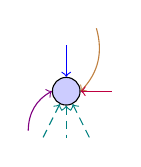
\begin{tikzpicture}[bt/.style = {<-, densely dashed, teal}]
  \node (n) [circle, minimum size = 10pt, draw, fill = blue!20] {};

  \draw[<-, blue] (n.north) to +(0, 0.4cm);	% tree edge
  \draw[<-, violet] (n.west) to[bend right] +(-0.3cm, -0.5cm);	% back edge
  \draw[<-, brown] (n.east) to[bend right] +(0.2cm, 0.8cm);	% forward edge
  \draw[<-, purple] (n.east) to +(0.4cm, 0cm);	% cross edge

  \path (n) edge[bt] +(0, -0.6cm)
	(n) edge[bt] +(-0.3cm, -0.6cm)
	(n) edge[bt] +(0.3cm, -0.6cm);
\end{tikzpicture}
\end{document}
